\documentclass[11pt,compress,t,notes=noshow, xcolor=table]{beamer}
\usepackage[]{graphicx}\usepackage[]{color}
% maxwidth is the original width if it is less than linewidth
% otherwise use linewidth (to make sure the graphics do not exceed the margin)
\makeatletter
\def\maxwidth{ %
  \ifdim\Gin@nat@width>\linewidth
    \linewidth
  \else
    \Gin@nat@width
  \fi
}
\makeatother

\definecolor{fgcolor}{rgb}{0.345, 0.345, 0.345}
\newcommand{\hlnum}[1]{\textcolor[rgb]{0.686,0.059,0.569}{#1}}%
\newcommand{\hlstr}[1]{\textcolor[rgb]{0.192,0.494,0.8}{#1}}%
\newcommand{\hlcom}[1]{\textcolor[rgb]{0.678,0.584,0.686}{\textit{#1}}}%
\newcommand{\hlopt}[1]{\textcolor[rgb]{0,0,0}{#1}}%
\newcommand{\hlstd}[1]{\textcolor[rgb]{0.345,0.345,0.345}{#1}}%
\newcommand{\hlkwa}[1]{\textcolor[rgb]{0.161,0.373,0.58}{\textbf{#1}}}%
\newcommand{\hlkwb}[1]{\textcolor[rgb]{0.69,0.353,0.396}{#1}}%
\newcommand{\hlkwc}[1]{\textcolor[rgb]{0.333,0.667,0.333}{#1}}%
\newcommand{\hlkwd}[1]{\textcolor[rgb]{0.737,0.353,0.396}{\textbf{#1}}}%
\let\hlipl\hlkwb

\usepackage{framed}
\makeatletter
\newenvironment{kframe}{%
 \def\at@end@of@kframe{}%
 \ifinner\ifhmode%
  \def\at@end@of@kframe{\end{minipage}}%
  \begin{minipage}{\columnwidth}%
 \fi\fi%
 \def\FrameCommand##1{\hskip\@totalleftmargin \hskip-\fboxsep
 \colorbox{shadecolor}{##1}\hskip-\fboxsep
     % There is no \\@totalrightmargin, so:
     \hskip-\linewidth \hskip-\@totalleftmargin \hskip\columnwidth}%
 \MakeFramed {\advance\hsize-\width
   \@totalleftmargin\z@ \linewidth\hsize
   \@setminipage}}%
 {\par\unskip\endMakeFramed%
 \at@end@of@kframe}
\makeatother

\definecolor{shadecolor}{rgb}{.97, .97, .97}
\definecolor{messagecolor}{rgb}{0, 0, 0}
\definecolor{warningcolor}{rgb}{1, 0, 1}
\definecolor{errorcolor}{rgb}{1, 0, 0}
\newenvironment{knitrout}{}{} % an empty environment to be redefined in TeX

\usepackage{alltt}
\newcommand{\SweaveOpts}[1]{}  % do not interfere with LaTeX
\newcommand{\SweaveInput}[1]{} % because they are not real TeX commands
\newcommand{\Sexpr}[1]{}       % will only be parsed by R
\newcommand{\xmark}{\ding{55}}%


\usepackage[english]{babel}
\usepackage[utf8]{inputenc}

\usepackage{dsfont}
\usepackage{verbatim}
\usepackage{amsmath}
\usepackage{amsfonts}
\usepackage{amssymb}
\usepackage{bm}
\usepackage{csquotes}
\usepackage{multirow}
\usepackage{longtable}
\usepackage{booktabs}
\usepackage{enumerate}
\usepackage[absolute,overlay]{textpos}
\usepackage{psfrag}
\usepackage{algorithm}
\usepackage{algpseudocode}
\usepackage{eqnarray}
\usepackage{arydshln}
\usepackage{tabularx}
\usepackage{placeins}
\usepackage{tikz}
\usepackage{setspace}
\usepackage{colortbl}
\usepackage{mathtools}
\usepackage{wrapfig}
\usepackage{bm}
\usepackage{amsmath}
\usepackage{pifont}
\usepackage{xcolor} %colored math symbols

\usetikzlibrary{shapes,arrows,automata,positioning,calc,chains,trees, shadows}
\tikzset{
  %Define standard arrow tip
  >=stealth',
  %Define style for boxes
  punkt/.style={
    rectangle,
    rounded corners,
    draw=black, very thick,
    text width=6.5em,
    minimum height=2em,
    text centered},
  % Define arrow style
  pil/.style={
    ->,
    thick,
    shorten <=2pt,
    shorten >=2pt,}
}

\usepackage{subfig}

% Defines macros and environments
\usepackage{../../style/lmu-lecture}


\let\code=\texttt
\let\proglang=\textsf

\setkeys{Gin}{width=0.9\textwidth}

\setbeamertemplate{frametitle}{\expandafter\uppercase\expandafter\insertframetitle}

\usepackage{bbm}
% basic latex stuff
\newcommand{\pkg}[1]{{\fontseries{b}\selectfont #1}} %fontstyle for R packages
\newcommand{\lz}{\vspace{0.5cm}} %vertical space
\newcommand{\dlz}{\vspace{1cm}} %double vertical space
\newcommand{\oneliner}[1] % Oneliner for important statements
{\begin{block}{}\begin{center}\begin{Large}#1\end{Large}\end{center}\end{block}}


%new environments
\newenvironment{vbframe}  %frame with breaks and verbatim
{
 \begin{frame}[containsverbatim,allowframebreaks]
}
{
\end{frame}
}

\newenvironment{vframe}  %frame with verbatim without breaks (to avoid numbering one slided frames)
{
 \begin{frame}[containsverbatim]
}
{
\end{frame}
}

\newenvironment{blocki}[1]   % itemize block
{
 \begin{block}{#1}\begin{itemize}
}
{
\end{itemize}\end{block}
}

\newenvironment{fragileframe}[2]{  %fragile frame with framebreaks
\begin{frame}[allowframebreaks, fragile, environment = fragileframe]
\frametitle{#1}
#2}
{\end{frame}}


\newcommand{\myframe}[2]{  %short for frame with framebreaks
\begin{frame}[allowframebreaks]
\frametitle{#1}
#2
\end{frame}}

\newcommand{\remark}[1]{
  \textbf{Remark:} #1
}


\newenvironment{deleteframe}
{
\begingroup
\usebackgroundtemplate{
\includegraphics[width=\paperwidth,height=\paperheight]{../style/color/red.png}}
 \begin{frame}
}
{
\end{frame}
\endgroup
}
\newenvironment{simplifyframe}
{
\begingroup
\usebackgroundtemplate{
\includegraphics[width=\paperwidth,height=\paperheight]{../style/color/yellow.png}}
 \begin{frame}
}
{
\end{frame}
\endgroup
}\newenvironment{draftframe}
{
\begingroup
\usebackgroundtemplate{
\includegraphics[width=\paperwidth,height=\paperheight]{../style/color/green.jpg}}
 \begin{frame}
}
{
\end{frame}
\endgroup
}
% https://tex.stackexchange.com/a/261480: textcolor that works in mathmode
\makeatletter
\renewcommand*{\@textcolor}[3]{%
  \protect\leavevmode
  \begingroup
    \color#1{#2}#3%
  \endgroup
}
\makeatother


\input{../../latex-math/basic-math}
\input{../../latex-math/basic-ml}
\input{../../latex-math/ml-nn}

\title{Deep Learning}
\date{}

\begin{document}
\newcommand{\titlefigure}{plots/unsupervised_3.png}
%modify picture
\newcommand{\learninggoals}{
  \item Unsupervised learning tasks
  \item Unsupervised deep learning
  %\item Principal component analysis
}

\lecturechapter{Unsupervised Learning}
\lecture{I2DL}



\begin{vbframe}{Unsupervised Learning}
  \begin{itemize}
    \item So far, we have described the application of neural networks to %upervised
     \textbf{supervised learning}  in which we have labeled training data $(\pmb{x}^{(1)}, \pmb{y}^{(1)}), \dots, (\pmb{x}^{(n)}, \pmb{y}^{(n)})$.
    \item In supervised learning scenarios
   we exploit label information (i.e. class memberships or numeric values) to train our algorithm. %That means in particular, that we have access to labeled data (y).
    \item% In supervised learning T
    The model learns a function to map $\pmb{x}$ to $\pmb{y}$.
    \item Examples are: classification, regression, object detection, semantic segmentation, image captioning, etc.
  \end{itemize}
    
        \begin{figure}
            \centering
            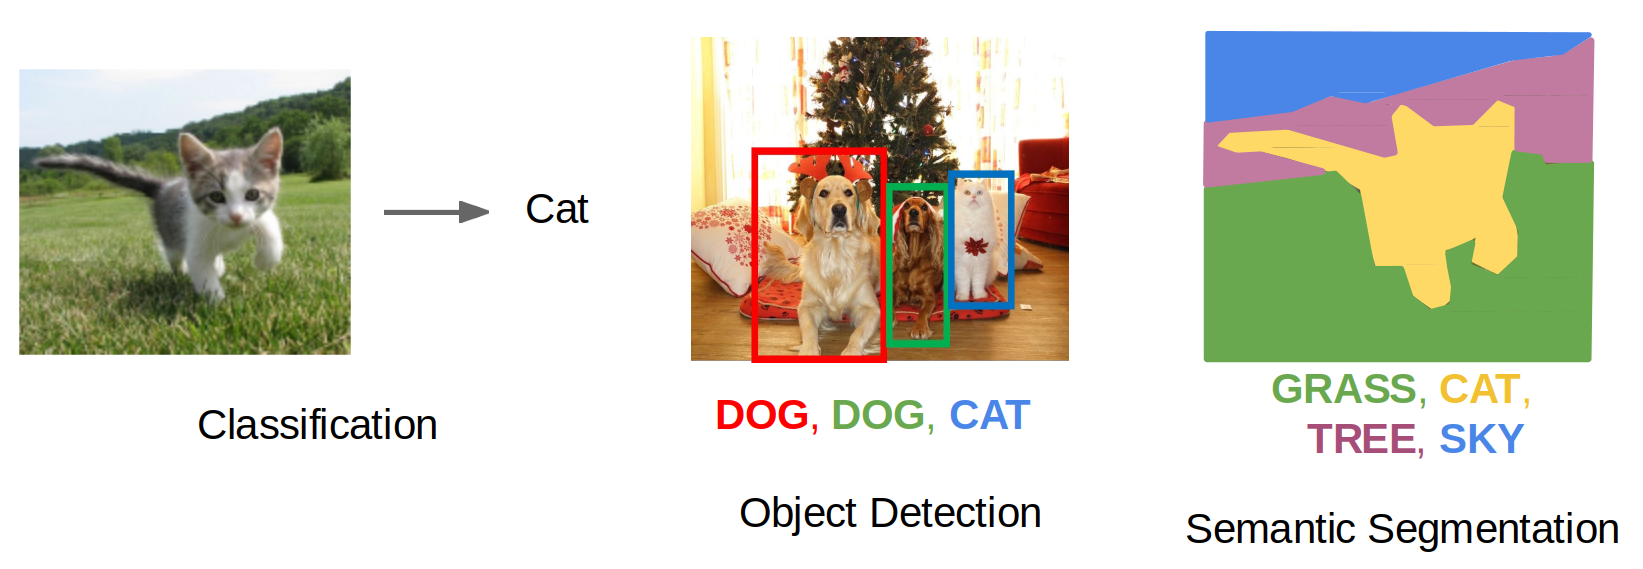
\includegraphics[width=0.6\linewidth]{plots/supervised.png}
           \caption{Examples of unsupervised learning (Li, 2023).}
        \end{figure}
    
    \framebreak
    
    \begin{itemize}
      \item In \textbf{unsupervised learning} scenarios
      %\item 
      training data consists of unlabeled input points $\pmb{x}^{(1)}, \dots, \pmb{x}^{(n)}$.
      \item Our goal is to learn some underlying hidden structure of the data.
      \item Examples are: clustering, dimensionality reduction, feature learning, density estimation, etc.
    \end{itemize}

\end{vbframe}

\begin{vbframe}{Unsupervised Learning - Examples}
  \begin{itemize}
    \item[] \textbf{1. Clustering.}
  \end{itemize}
  \begin{figure}
    \centering
    \scalebox{1}{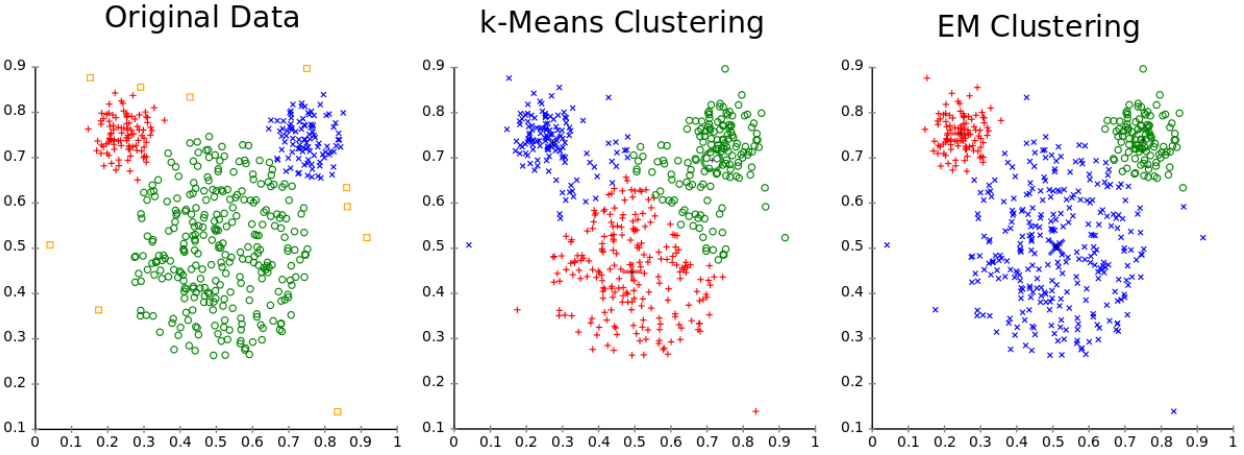
\includegraphics{plots/clustering_2.png}}
    \caption{Cluster analysis results  for different algorithms. Different clusters are indicated by different colors  (Bullibabu et al., 2016).}
  \end{figure}
\framebreak
  \begin{itemize}
    \item[] \textbf{2. Dimensionality reduction/manifold learning.}
    \ \begin{itemize}
    \item E.g.~for visualisation in a low dimensional space.
    \end{itemize}
  \end{itemize}

    \begin{figure}
        \only<1-2>{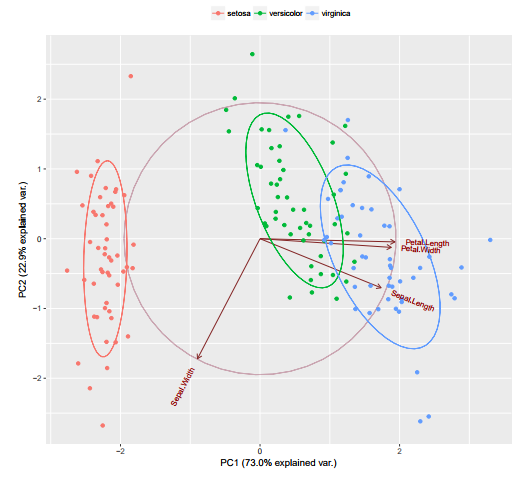
\includegraphics[width=6.cm]{plots/unsupervised_3.png}}
        \caption{Principal Component Analysis (PCA) (Finnstats, 2021).}
    \end{figure}

\framebreak
  \begin{itemize}
    \item[] \textbf{2. Dimensionality reduction/manifold learning.}
    \ \begin{itemize}
    \item E.g.~for  image compression.
    \end{itemize}
  \end{itemize}

    \begin{figure}
        \only<1-2>{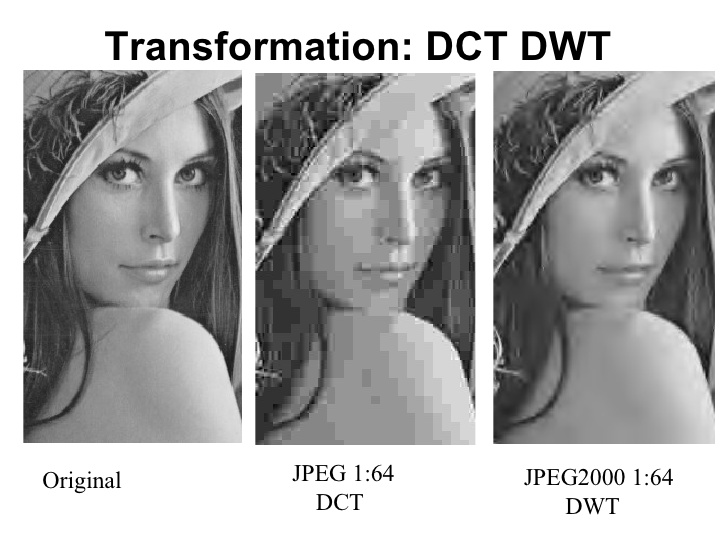
\includegraphics[width=5.cm]{plots/imagecompression.jpg}}
        \caption{Example of image compression (Cycon, 2009).}
    \end{figure}

\end{vbframe}



\begin{vbframe} {Unsupervised Learning - Examples}
  \begin{itemize}
    \item[] \textbf{3. Feature extraction/representation learning.}
    \item[]
  \end{itemize}
   \begin{figure}
        \only<1-2>{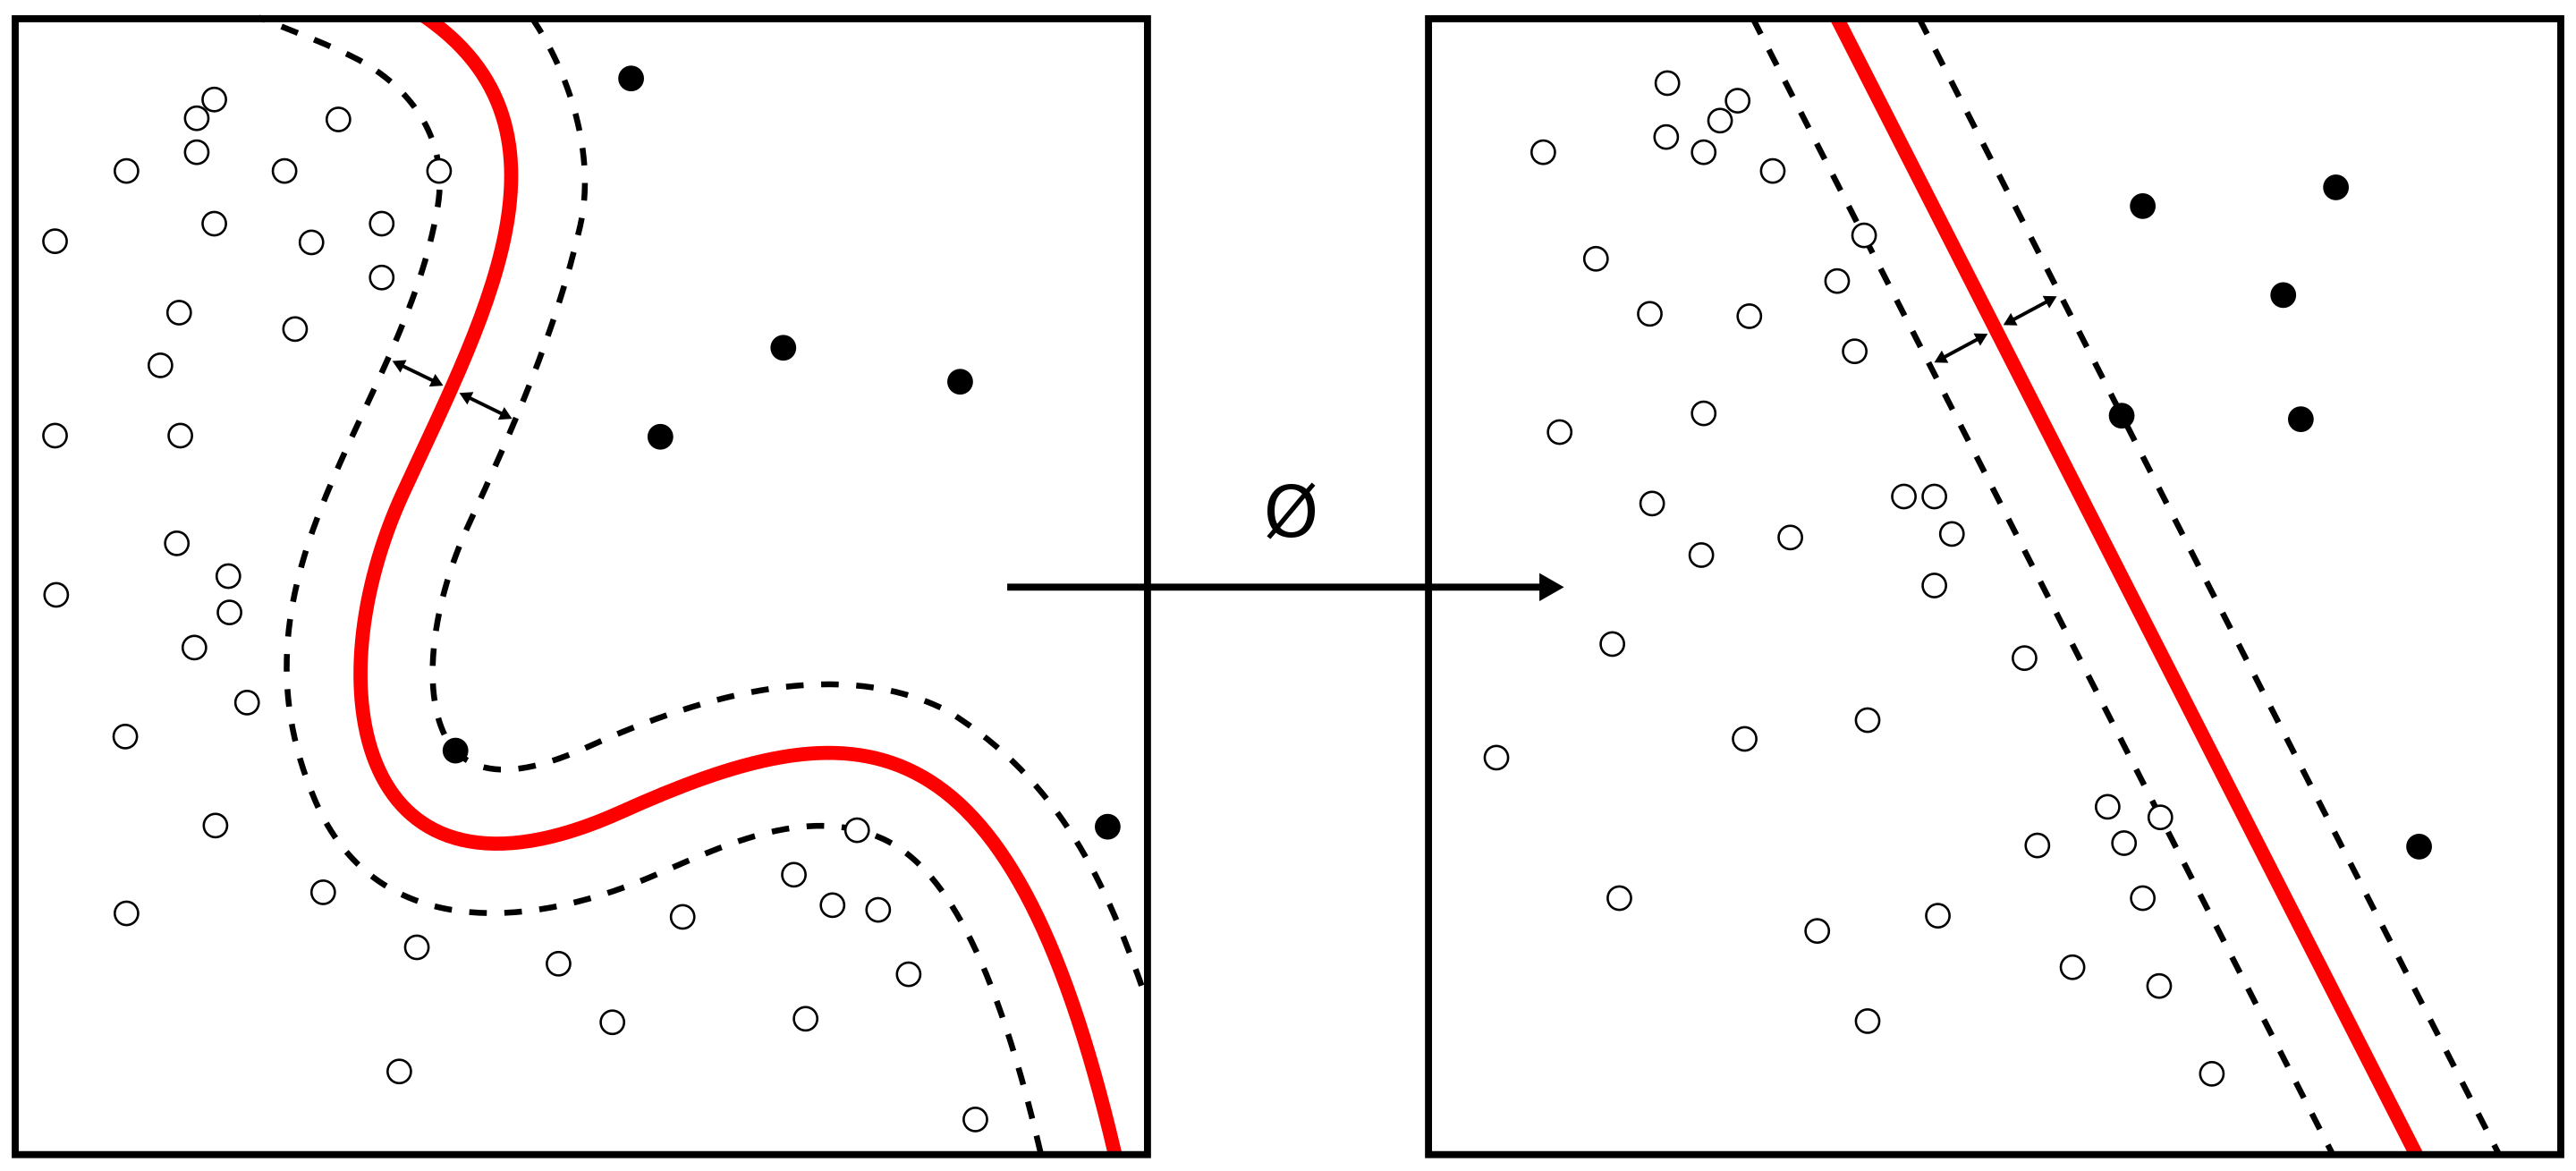
\includegraphics[width=4.cm]{plots/feature_extraction.png}}
        \caption{Use of kernel machines to obtain a linearly separable function (Matzer, 2019).}
    \end{figure}
    \begin{itemize}
    \item  E.g.~for \textbf{semi-supervised learning}: features learned from an unlabeled dataset are employed to improve performance in a supervised setting. 
    \end{itemize}
\framebreak
  \begin{itemize}
    \item[] \textbf{4. Density fitting/learning a generative model.}
    \item[]
  \end{itemize}
   \begin{figure}
        \only<1-2>{\scalebox{1}{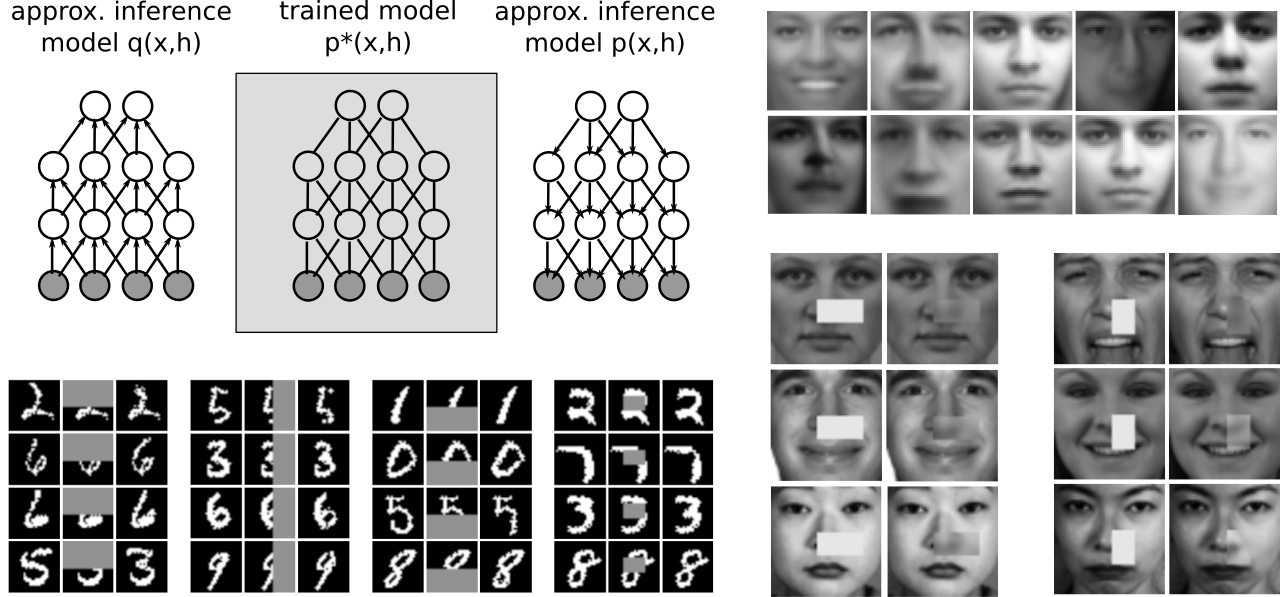
\includegraphics{plots/BHM.png}}}
        \caption{A generative model can reconstruct the missing portions of the images (Bornschein et al., 2016).}
    \end{figure}
    

\end{vbframe}


%%%%%%%%%%%%%%%%%%%%%%%%%%%%%%%%%%%%%%%%%%%%%%%%%%%%%%%%%%%%%%%%%%%%%%%%%
%\begin{vbframe}
%\frametitle{Manifold learning}

%  \begin{itemize}
%        \item \textbf{Manifold hypothesis}: 
%        Data of interest lies on an embedded non-linear manifold within the higher-dimensional space.
    %    Data is concentrated around a low-dimensional \textit{manifold} or a small set of such manifolds
        %    \pause
        % \item In mathematics, a manifold is a topological space that locally resembles Euclidean space near each point 
 %       \item A \textbf{manifold}: 
%        \begin{itemize}
%        \item  is a topological space that locally resembles the Euclidean space.
%        \item  in ML, more loosely refers to a connected set of points that can be approximated well by considering only a small number of dimensions. 
 %       \end{itemize}
 %         \begin{figure}[h]
 %               \centering
%                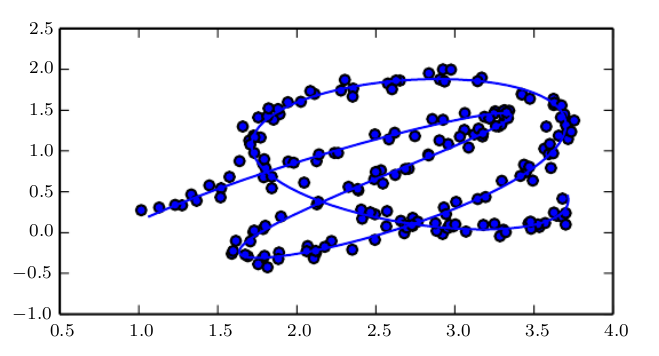
\includegraphics[width=5  cm]{plots/manifold.png}
%                \caption{
%                from Goodfellow et. al%Data sampled from a distribution in a 2D space that is actually concentrated near a 1D manifold.
%                }
%            \end{figure}
%           \end{itemize}    
%       \framebreak
 
%\begin{itemize}
%    \item An important characterization of a manifold is the set of its tangent planes.
%    \item \textbf{Definition}: At a point $\pmb{x}$ on a $d$-dimensional manifold, the \textbf{tangent plane} is given by $d$ basis vectors that span the local directions of variation allowed on the manifold.
    
%\end{itemize} 
%        \begin{figure}[h]
 %           \centering
%            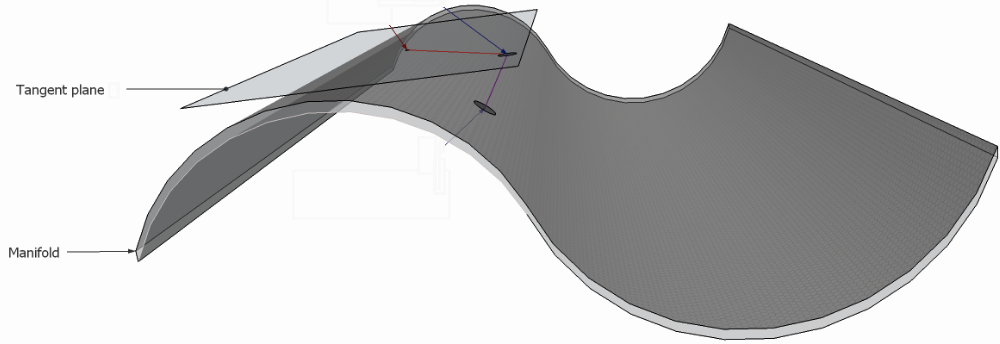
\includegraphics[width=0.8\linewidth]{plots/tangent_plane.png}
%            \caption{A pictorial representation of the tangent space of a single point, \textbf{\textit{x}}, on a manifold (Goodfellow et al. (2016)).}
%        \end{figure}
     
 %      \framebreak
       
      
%        \begin{itemize}
%        \item Manifold hypothesis does not need to  hold true.
        %assumption that the data lies along a low-dimensional manifold may notalways be correct
 %       \item In the context of AI tasks (e.g.~processing images, sound, or text) it seems to be at least approximately correct, since :
%        \begin{itemize}
 %       \item probability distributions over images, text strings, and sounds that occur in real life are highly concentrated (randomly sampled pixel values do not look like images, randomly sampling letters is unlikely to result in a meaningful sentence).
 %       \item samples are connected to each other by other samples, with each sample surrounded by other highly similar samples that can be reached by applying transformations (E.g. for images, dim or brighten the lights, move or rotate objects, change the colors of objects,  etc).
 %    \end{itemize}
      % TODO: add more on the manifold view ?
 %   \end{itemize} 

%\end{vbframe}


%%%%%%%%%%%%%%%%%%%%%%%%%%%%%%%%%%%%%%%%%%%%%%%%%%%%%%%%%%%%%%%%%%
%\begin{vbframe}{Revision of PCA}
%\begin{itemize}
%  \item The purpose of PCA is to project the data $\mathbf{x}^{(1)}, \dots, \mathbf{x}^{(n)}$ onto a lower-dimensional subspace (e.g. to save memory). \\
%  \item For each point $\mathbf{x}^{(i)} \in \mathbb{R}^p$ we need to find a corresponding code vector $\mathbf{c}^{(i)} \in \mathbb{R}^l$ with $l < p$. That step is accomplished by the encoding function which produces the code for an input: $$f(\mathbf{x}) = \mathbf{c}$$
%  \item  Additionally, we need a decoding function to produce the reconstruction of the input given its code: $$\mathbf{x} \approx g(f(\mathbf{x}))$$
%  \item PCA is then defined by the choice of the encoding and decoding function.
%  \item We can choose matrix multiplication to map the data back into $\mathbb{R}^{p}$: $g(\mathbf{c}) = \mathbf{Dc}$, with $\mathbf{D} \in \mathbb{R}^{p \times l}$, defining the decoding.
%\framebreak
%  \item To keep the encoding problem easy, PCA constrains the columns of $\mathbf{D}$ to be orthogonal.
%  \item We begin with the optimal code $\mathbf{c}^{*}$ for each input. We could achieve this by minimizing the distance between the input $\mathbf{x}$ and its reconstruction $g(\mathbf{c})$ (PCA is a linear transformation with minimum reconstruction error)
%  \item One way to obtain the optimal code $\mathbf{c}^{*}$ is to minimize the distance between the input $\mathbf{x}$ and its reconstruction $g(\mathbf{c})$ (that means, linear transformation with minimum reconstruction error):
%   $$\mathbf{c}^{*} = \displaystyle\argmin_{\mathbf{c}} ||\mathbf{x} - g(\mathbf{c})||^2_2$$
%  \item Solving this optimization problem leads to
%  $$\mathbf{c} = \mathbf{D}^T\mathbf{x}$$
%  \item Thus, to encode a vector, we apply the encoder function
%  $$f(\mathbf{x}) = \mathbf{D}^T \mathbf{x}$$
% \framebreak
% \begin{itemize}
%  \item
%  We can also define the PCA as the reconstruction operation:
%  $$r(\mathbf{x}) = g(f(\mathbf{x})) = \mathbf{DD}^T \mathbf{x}$$
%\end{itemize}
%   \item To find the encoding matrix $\mathbf{D^*}$, we minimize the Frobenius norm of the matrix of errors computed over all dimensions and points:
%   $$\mathbf{D^*} = \displaystyle\argmin_{\mathbf{D}} \sqrt{\displaystyle\sum_{i,j} \Big(x^{(i)}_j - r(x^{(i)})_j\Big)^2}, \text{ subject to } \mathbf{D^T}\mathbf{D} = \mathbf{I}_l$$
%   \item for $l = 1$, $\mathbf{D^*}$ collapses to a single vector and we can rewrite the equation as
%   $$\mathbf{d^*} = \displaystyle\argmin_{\mathbf{d}} ||\mathbf{X} - \mathbf{X}\mathbf{d}\mathbf{d}^T||^2_F, \text{ subjected to } \mathbf{d}^T\mathbf{d} = 1$$
%   \item The optimal $\mathbf{d^*}$ is given by the eigenvector of $\mathbf{X}^T\mathbf{X}$ corresponding to the largest eigenvalue.
% \end{itemize}
% \framebreak  
% \begin{itemize}
%   \item In general, for $l = k$ (with $k < p$) , the optimal reconstruction $\mathbf{X}^*$, by the Eckart-Young-Mirsky Theorem, is the truncated \textbf{Singular Value Decomposition (SVD)} of $\mathbf{X}$ :
%   $$
% \mathbf{X}^* = \mathbf{U}_k \boldsymbol{\Sigma}_k \mathbf{V}_k^\top
% $$
% where, the diagonal matrix $\boldsymbol{\Sigma}_k$ contains the $k$ largest \textbf{singular values} and the columns of the matrices $\mathbf{U}_k$ and $\mathbf{V}_k$ are the corresponding \textbf{right singular vectors} and \textbf{left singular vectors}, respectively.
% \item Here, the optimal encoding matrix $\mathbf{D}^*$ consists of the $k$ left singular vectors as columns.
% \end{itemize}
% \framebreak
% \begin{itemize}
%   \item \small{The first principal component has the largest possible variance (that is, accounts for as much of the variability in the data as possible).
%   
%   \item Each succeeding component in turn has the highest variance possible under the constraint that it is orthogonal to the preceding components.}
% 
%  \begin{figure}
%     \centering
%     \scalebox{0.6}{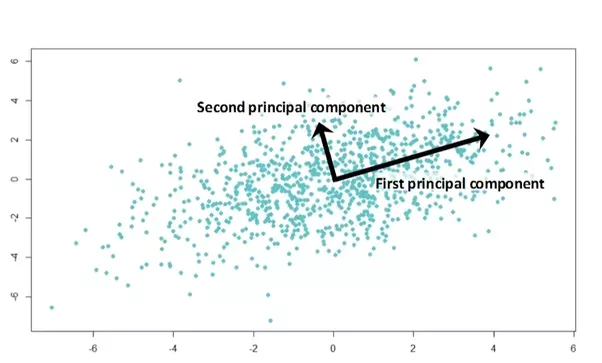
\includegraphics{plots/PCA_1.png}}
%     \tiny{\\credit:Syed Nazrul}
%       \caption{\footnotesize{The vectors shown are the (scaled) eigenvectors. Keeping only the first principal component results in dimensionality reduction.}}
%   \end{figure}
%   \end{itemize}
  
%\end{vbframe}

%%%%%%%%%%%%%%%%%%%%%%%%%%%%%%%%%%%%%%%%%%%%%%%%%%%%%%%%%%%%%%%%%%
\begin{frame}[fragile]
\frametitle{Unsupervised Deep Learning}
Given i.i.d. (unlabeled) data $\mathbf{x}_1, \mathbf{x}_2,\dots, \mathbf{x}_n \sim  p_{\text{data}}$, 
 in unsupervised deep learning, one usually trains :

 \begin{itemize}
 
 \item  an autoencoder (a special kind of neural network) for \textbf{representation learning} (feature extraction, dimensionality reduction, manifold learning, ...), or, \\
 %$\righarrow$ This neural networks are 

 \pause
 
  \item a \textbf{generative model}, i.e.~a probabilistic model of the  data generating distribution  $p_{\text{data}}$ 
  % (predictions, missing feature estimation, reconstruction, denoising, sampling, outlier detection, ...).
  (data generation, outlier detection, missing feature extraction, reconstruction, denoising or planning in reinforcement learning, ...). 
  
  %full probabilistic model of all variables
  
 \end{itemize}

\end{frame} 
%%%%%%%%%%%%%%%%%%%%%%%%%%%%%%%%%%%%%%%%%%%%%%%%%%%%%%%%%%%%%%%
%%%%%%%%%%%%%%%%%%%%%%%%%%%%%%%%%%%%%%%%%%%%%%%%%%%%%%%%%%%%%%%%%%
%%%%%%%%%%%%%%%%%%          REFERENCES          %%%%%%%%%%%%%%%%%%
%%%%%%%%%%%%%%%%%%%%%%%%%%%%%%%%%%%%%%%%%%%%%%%%%%%%%%%%%%%%%%%%%%
\begin{vbframe}
\frametitle{References}
\footnotesize{
\begin{thebibliography}{99}
%%%%%%%%%%%%%%%%%%%%%%%%%%%%%%%%%%
\bibitem[(Bornschein et al., 2016)]{1} Bornschein, J., Shabanian, S., Fischer, A., \& Bengio, Y. (2016). \textit{Bidirectional Helmholtz Machines}.
%%%%%%%%%%%%%%%%%%%%%%%%%%%%%%%%%%
\bibitem[(Cycon, 2009)]{2} Cycon. (2009, May 4). \textit{Bildkompression}. PPT. \url{https://de.slideshare.net/hcycon/bildkompression} 
%%%%%%%%%%%%%%%%%%%%%%%%%%%%%%%%%%
\bibitem[(Matzer, 2019)]{3} Matzer, M. (2019, April 29). \textit{Optimale clusteranalyse und segmentierung mit dem k-means-algorithmus}. BigData. \url{https://www.bigdata-insider.de/optimale-clusteranalyse-und-segmentierung-mit-dem-k-means-algorithmus-a-773713/}
%%%%%%%%%%%%%%%%%%%%%%%%%%%%%%%%%%
\bibitem[(Finnstats, 2021)]{4} Finnstats. (2021, May 7). \textit{Principal Component Analysis (PCA) in R: R-bloggers. R-bloggers}. \url{https://www.r-bloggers.com/2021/05/principal-component-analysis-pca-in-r/} 
%%%%%%%%%%%%%%%%%%%%%%%%%%%%%%%%%
\bibitem[(Bullibabu et al., 2016)]{5} Bullibabu, Rasamsetty \& Snehal, G. \& Kiran, P.. (2016). \textit{Detection of Crimes using Unsupervised Learning Techniques}. Indian Journal of Science and Technology. 
%%%%%%%%%%%%%%%%%%%%%%%%%%%%%%%%
\bibitem[(Li, 2023)]{6} Li, F.-F. (2023). \textit{Lecture 11: Detection and segmentation - Stanford University}. CS231n. \url{http://cs231n.stanford.edu/slides/2017/cs231n_2017_lecture11.pdf}

\end{thebibliography}
}
\end{vbframe}



\endlecture
\end{document}
